\documentclass{article}
\usepackage{enumitem, amsmath, amssymb, mathtools, titlesec}
\usepackage[margin = 1in]{geometry}

\titlespacing\section{0pt}{0pt}{-8pt}

\newcommand{\T}{\top}
\newcommand{\dpd}[2]{\dfrac{\partial #1}{\partial #2}}
\newcommand{\dpdop}[1]{\dfrac{\partial}{\partial #1}}
\renewcommand{\vec}[1]{\mathbf{#1}}

\DeclarePairedDelimiter{\p}{(}{)}
\DeclarePairedDelimiter{\set}{\{}{\}}
\DeclarePairedDelimiter{\norm}{\Vert}{\Vert}

\DeclareMathOperator{\cs}{span}

\setlength{\parindent}{0pt}
\setlength{\parskip}{\bigskipamount}

\begin{document}

{\huge Lab Assignment 1} \\	
\large Steven Truong

\section*{Task 1}
First note that
\[
	\vec{z}_n^\T\vec{w} = \sum_{i=0}^{M-1} w_ix_n^i
\]
which is linear in each $w_i$. Then
\begin{align*}
	\dpd{J\p{\vec{w}}}{w_i} &= \dpdop{w_i}\p*{\frac{1}{2}\sum_{n=1}^N \p{\vec{z}_n^\T\vec{w} - t_n}^2} \\
	&= \sum_{n=1}^N \p{\vec{z}_n^\T\vec{w} - t_n}x_n^i.
\end{align*}
This gives us the following gradient:
\[
	\nabla J\p{\vec{w}} = \sum_{n=1}^N \p{\vec{z}_n^\T\vec{w} - t_n}\vec{z}_n
\]
Then
\begin{align*}
	\nabla J\p{\vec{w}} = \vec{0} &\iff \sum_{n=1}^N \p{\vec{z}_n^\T\vec{w} - t_n}\vec{z}_n = \vec{0} \\
	&\iff \sum_{n=1}^N \vec{z}_n\vec{z}_n^\T\vec{w} = \sum_{n=1}^N t_n\vec{z}_n \\
	&\iff A\vec{w} = \vec{b},
\end{align*}
where
\[
	A = \sum_{n=1}^N \vec{z}_n\vec{z}_n^\T \qquad\text{and}\qquad \vec{b} = \sum_{n=1}^N t_n\vec{z}_n.
\]

\pagebreak
\section*{Task 2}
Note that
\[
	\renewcommand{\arraystretch}{1.5}
	\begin{pmatrix}
 		\vec{z}_1^\T \\ \vec{z}_2^\T \\ \vdots \\ \vec{z}_N^\T
 	\end{pmatrix}
\]
is the Vandermonde matrix, which we'll call $V$. Also, it is known that $V$ is always full rank as long as all the $x_n$ are different. This means that the $\vec{z}_n$ are linearly independent if $N < M$.

There will always be a solution to the system $A\vec{w} = \vec{b}$, and uniqueness depends on $M$ and $N$. There are two cases to consider.

Case 1: $N < M$ \\
In this case, solutions are not unique. For $N < M$, the $\vec{z}_n$ are linearly independent, so we have
\[
	J\p{\vec{w}} = \vec{0} \iff \vec{z}_n^\T\vec{w} - t_n = 0\ \forall n
\]
which, written in matrix form, is $V\vec{w} = \vec{t}$, where $\vec{t} = \begin{pmatrix} t_1 & t_2 & \cdots & t_N \end{pmatrix}^\T$, and $V$ is full row rank. $V$ is thus onto, but not one-to-one, which means that we have non-unique solutions for all $\vec{t}$.

Case 2: $N \geq M$ \\
We'll show that $A$ is positive definite, so it's bijective. In other words, for every $\vec{b}$, there exists a unique $\vec{w}$ satisfying $A\vec{w} = \vec{b}$.

$A$ is positive semidefinite since it is the sum of positive semidefinite matrices. Suppose there exists some $\vec{z} \neq \vec{0}$ such that $\vec{z}^\T A\vec{z} = 0$. Then since each $\vec{z}_n\vec{z}_n^\T$ is positive semidefinite,
\[
	\vec{z}^\T A\vec{z} = \sum_{n=1}^N \vec{z}^\T\p*{\vec{z}_n\vec{z}_n^\T}\vec{z} = 0 \iff \vec{z}^\T\p*{\vec{z}_n\vec{z}_n^\T}\vec{z} = 0\ \forall n.
\]
Since $\vec{z}$ is not the zero vector, $\vec{z}$ must be orthogonal to $\vec{z}_n$ for all $n$. But since $N \geq M$ and $V$ has full rank, $\set{\vec{z}_1, \ldots, \vec{z}_N}$ spans $\mathbb{R}^M$. This implies that $\vec{z}$ must be $\vec{0}$ since it will be orthogonal to every vector in $\mathbb{R}^M$ since any vector can be written as a linear combination of $\set{\vec{z}_1, \ldots, \vec{z}_N}$, which is a contradiction. Thus, $A$ is positive definite, so $A\vec{w} = \vec{b}$ has a unique solution for any $\vec{b}$.

\pagebreak
\section*{Task 4}
\begin{figure}[h]
	\centering
	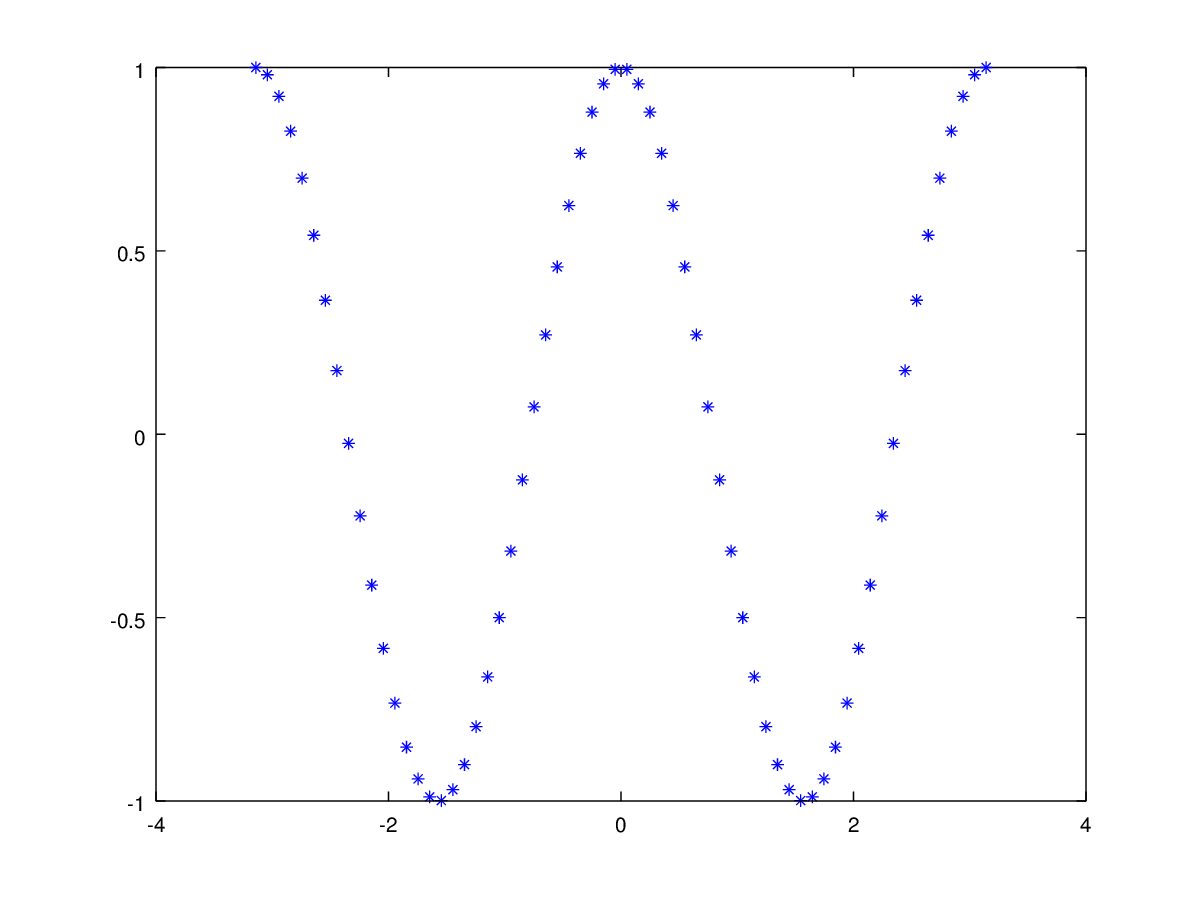
\includegraphics[width = 0.4\textwidth]{images/data}
\end{figure}

\section*{Task 6}
$M = 4$ gives a poor approximation of our data since it's unable to capture the oscillation of $f$ at all.

$M = 8$ gives a decent approximation of our data. It's able to capture the oscillation of $f$ on the interval of interest, and it matches the overall shape of our sample. However, it's not able to capture the peaks very well, especially at the origin.

$M = 16$ gives, by far, the best approximation of the data. It pretty much fits the data set exactly.

$M = 32$ is also a good approximation of the data, but not as well as $M = 16$. It fits the data extremely well except at the ends of the interval, where it begins to explode because of its large degree.

$M = 64$ is mostly the same as $M = 32$, but it explodes much faster at the end points than $M = 32$, and in the opposite direction.

\section*{Task 7}
\begin{figure}[h]
	\centering
	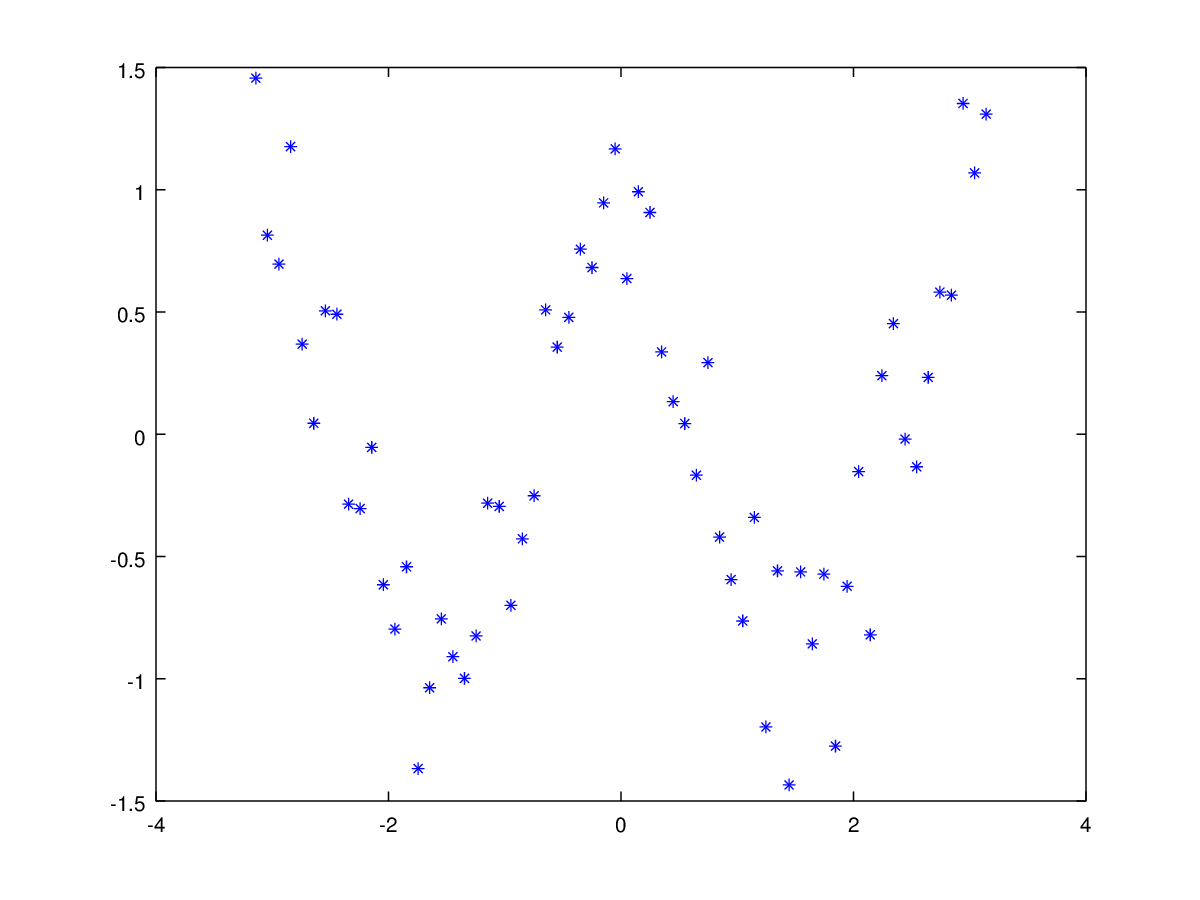
\includegraphics[width = 0.4\textwidth]{images/data-noise}	
\end{figure}

\pagebreak
\section*{Task 8}
$M = 4$ doesn't give a very good approximation of the data since it's unable to capture the oscillation of $f$.

$M = 8$ and $M = 16$ are the best approximations for the data sample from our tested polynomials. However, $M = 16$ seems to be the best overall since their key difference is that $M = 16$ captures the peak at the origin better than $M = 8$.
	
When $M$ is close to $N$, we get graphs that oscillate and explode close to the ends of our sample. This is true for $M = 32$ and $M = 64$, which both oscillate and have sharp jumps in the graph. For example, close to $x = -3$, $M = 64$ has a huge jump right before it explodes.

\begin{minipage}[t]{0.5\textwidth}
	\centering
	$M = 4$ \\
	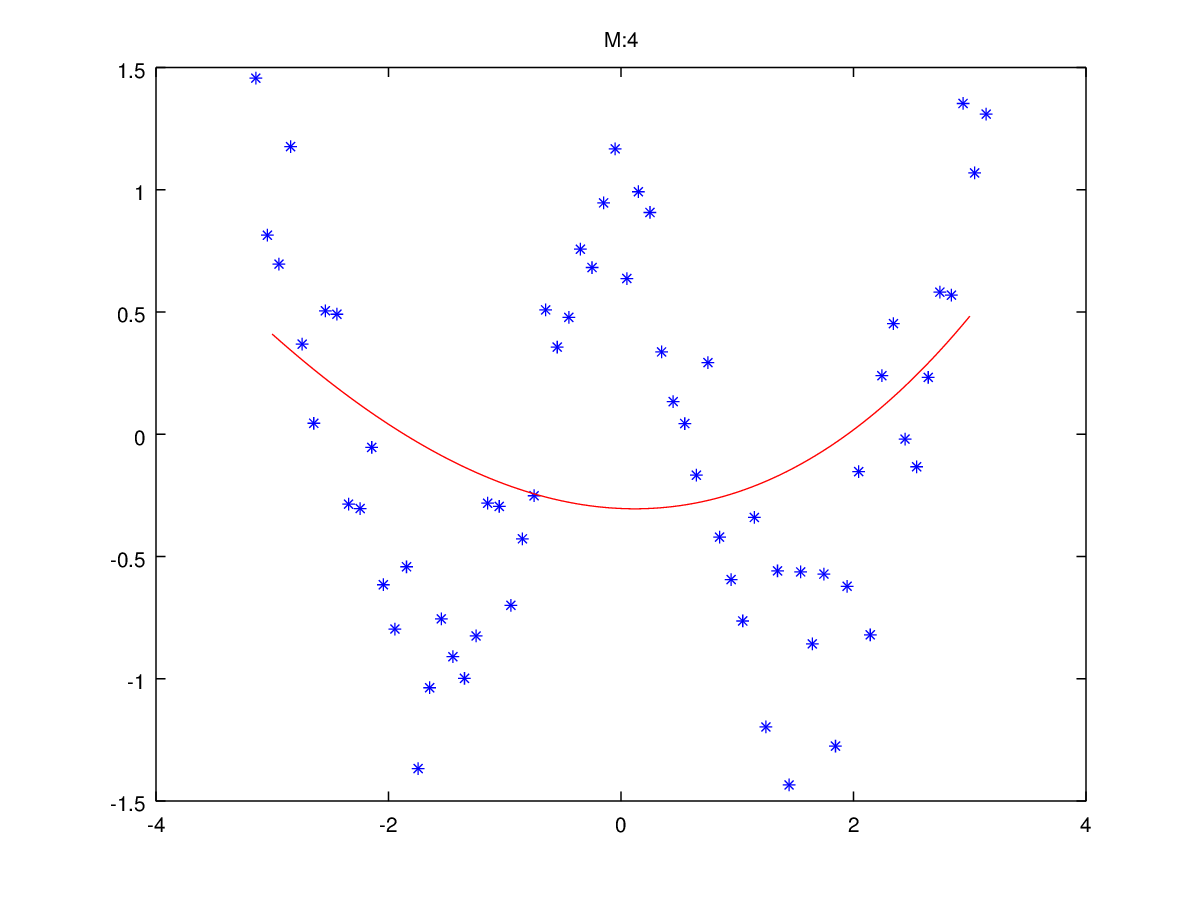
\includegraphics[width = 0.8\textwidth]{images/4}
	
	$M = 8$ \\
	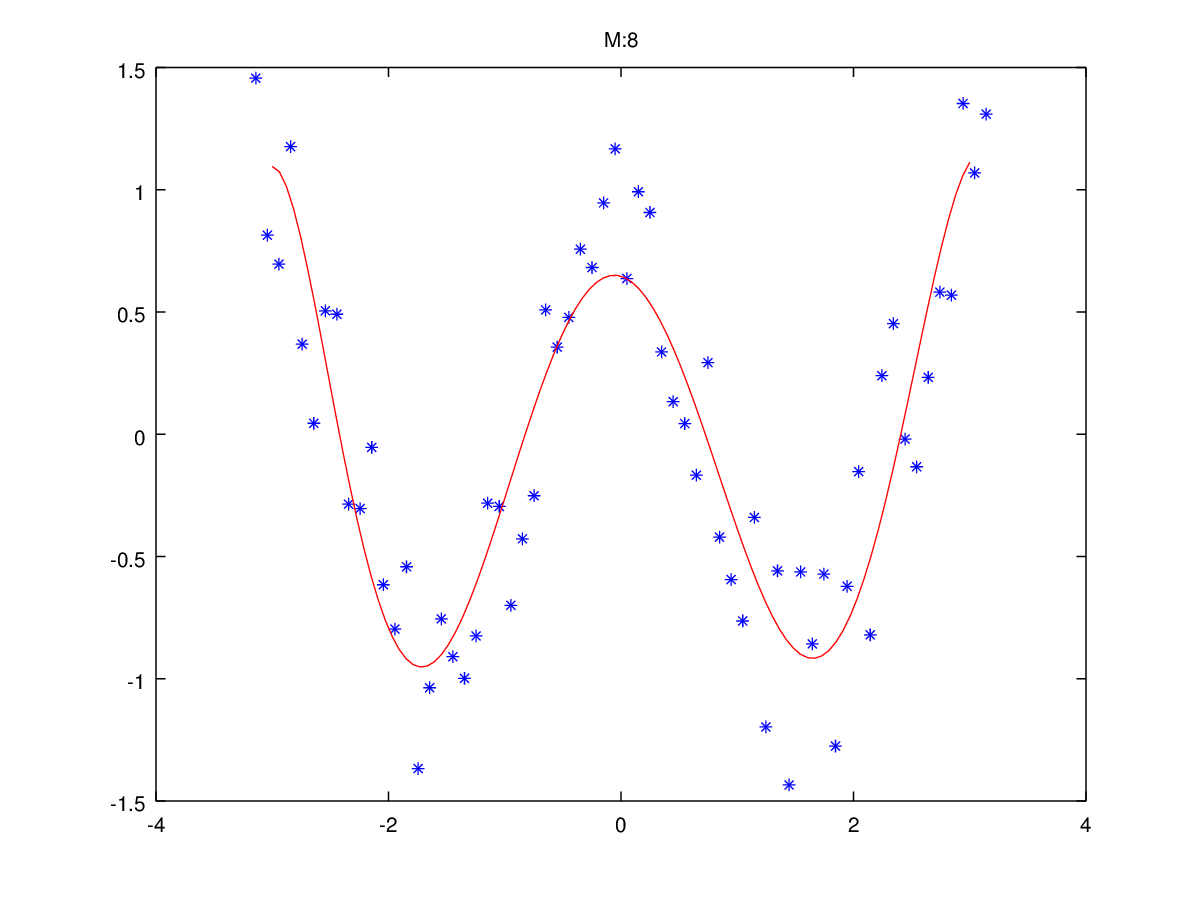
\includegraphics[width = 0.8\textwidth]{images/8}
	
	$M = 16$ \\
	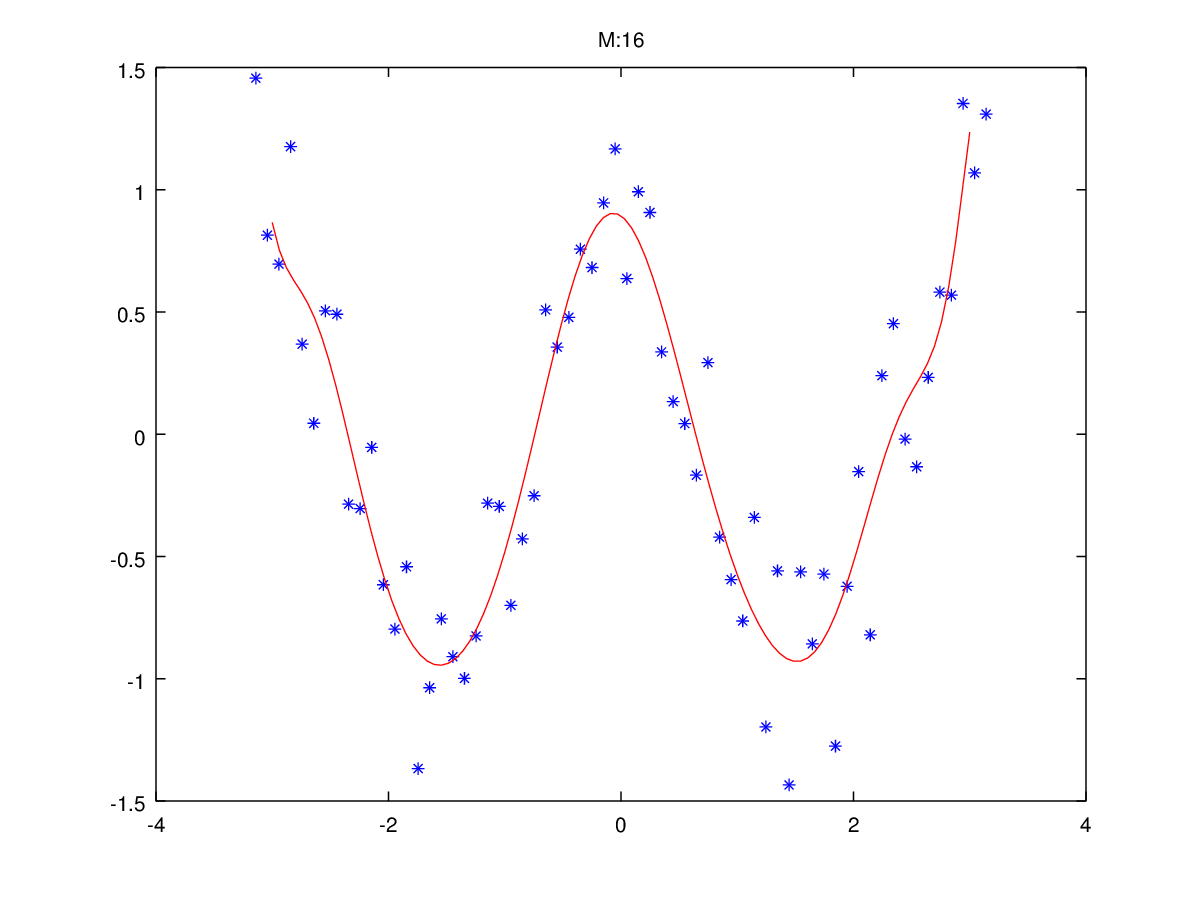
\includegraphics[width = 0.8\textwidth]{images/16}
\end{minipage}
\begin{minipage}[t]{0.5\textwidth}
	\centering
	$M = 32$ \\
	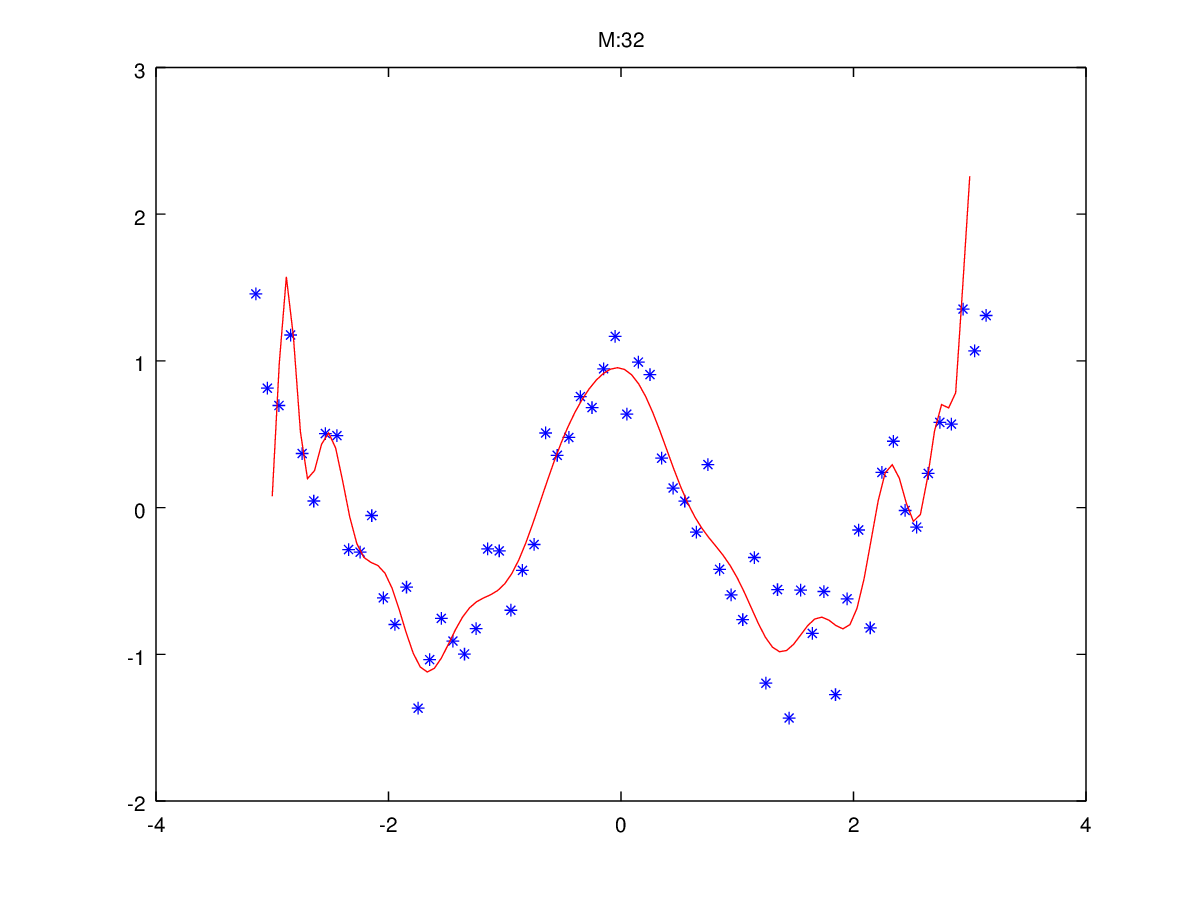
\includegraphics[width = 0.8\textwidth]{images/32}
	
	$M = 64$ \\
	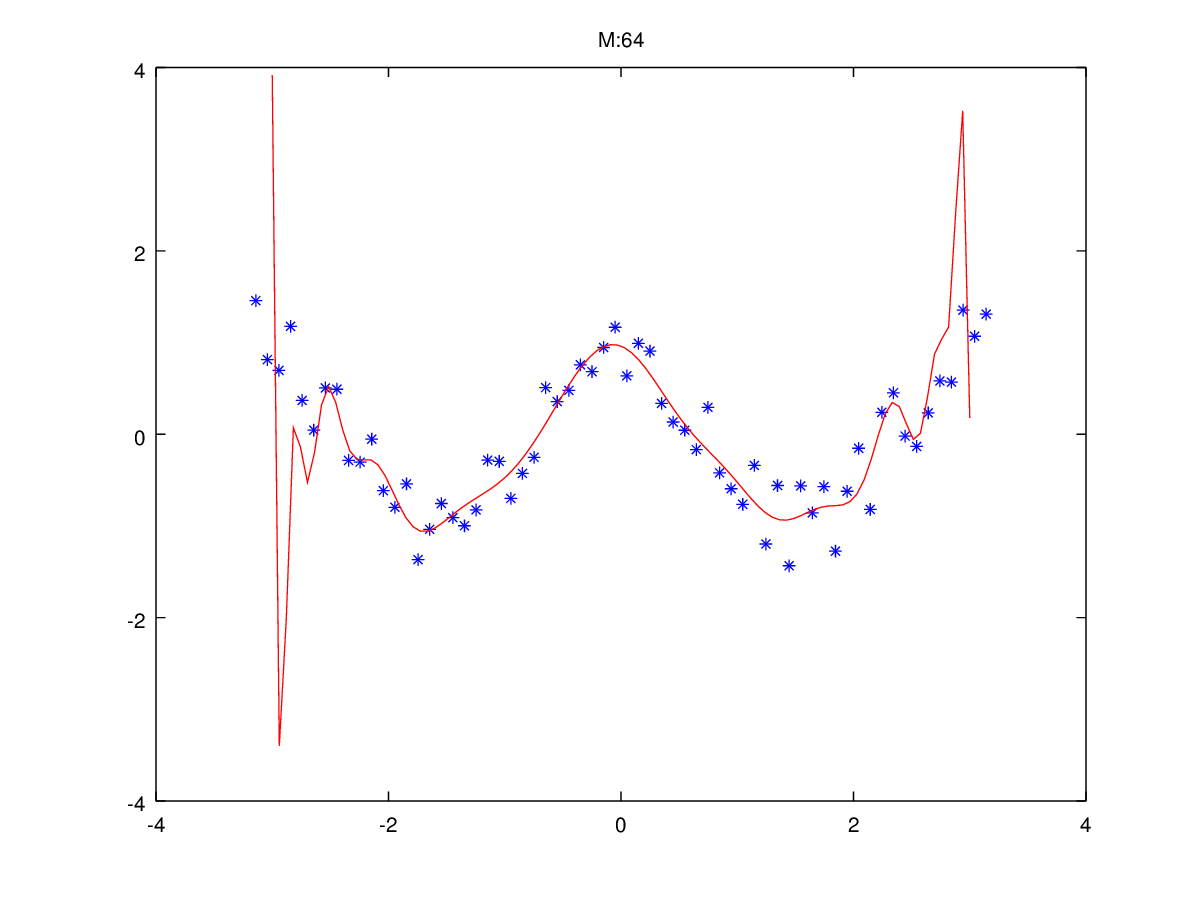
\includegraphics[width = 0.8\textwidth]{images/64}
\end{minipage}

\end{document}
